\documentclass{article}

\usepackage{graphicx}
\usepackage{amsmath}
\usepackage{braket}
\usepackage{float}
\usepackage[margin=1in]{geometry}


\def\hwtitle{How the Transients Simulations Work}
\def\hwauthor{Sarah Chastain}
%\def\hwdate{Jan. 24, 2020}

\usepackage{fancyhdr}
\lhead{\hwauthor}
\chead{\hwtitle}
\rhead{\date}
\lfoot{\hwauthor}
\cfoot{\today}
\rfoot{\thepage}
\renewcommand{\footrulewidth}{0.4pt}
\pagestyle{fancy}
%
\author{\hwauthor}
\title{\hwtitle}
\date{\today}

\begin{document}
	
	\maketitle
	\thispagestyle{fancy}
	
	
\section{Input and Configuration}
Before running the code it is necessary to provide some input in terms of both the observation set up and in the simulation parameters. For this purpose, the code reads in one or perhaps two files:
\subsection{config.ini}
This file is required. It contains two sections.
\subsubsection{Initial Parameters}
These are the parameters to be used for the simulations themselves. See the commented file for more details of what each parameter is. 
\subsubsection{Simulation Parameters (Sim)}
If there is no provided file with observation details, then this section contains the observation parameters.
\subsection{Observation file}
This file is optional. It contains the details of the observations in a list with columns.

\section{Parsing the Input}
The code then parses the input supplied from the command line and the input files listed above. The command line options include the option to only do the simulation calculations, to only plot the results, and to save all of the intermediate steps.
\section{Observation Parameters}
 The code then converts the inputted observation parameters into a usable format for the rest of the code in the ``observing\_strategy'' function. 
 \section{Generating Simulated Sources}
 Then, provided the users desires the simulations be calculated, this is passed on to a function that generates simulated sources. 
 \subsection{Durations}
 The first step is to generate durations that are randomly selected from a logarithmically uniformly spaced distribution of durations from the specified minimum to the specified maximum.
 \subsection{Fluxes}
 Next, the fluxes are simulated, yet again, from a logarithmically uniformly spaced distribution of fluxes from the specified minimum to the specified maximum.
 \subsection{Start Times}
 The sources are given a randomized start time that depends on the duration along with some of the observation parameters. Since the beginnings of these light curves are immediate in time, the only transients that will be detected are those which start before the end of the observation period. However, the transients may start before the beginning of the first observation. As far back as one transient duration before the first observation began. Therefore, the start time will be randomly chosen to be between one duration before the start of the observations and the end of observations.
\section{Detection of Simulated Sources}
These simulated sources are then run through a function that determines whether they are detected in the observations. The idea is to iterate over the observations and in each observation look to see what sources are detected. We follow the section criteria in the following sections.
\subsection{Edge Cases}
The first step in determining which simulated sources are candidates. The three implemented light curve types have different approaches:
\subsubsection{FRED}
The start time of the sources must not be equal to the end of the observation.
\subsubsection{Tophat}
There are two conditions: the source must not start and end before or right at the start of observations and the source must not start at the end of the observation.
\subsubsection{Gaussian}
We do no additional conditions here since this light curve has already had sufficient conditions imposed.
\subsection{Integrated Flux Filtering}
We now add some randomized errors to the peak flux that we simulated. Then we integrate over the observation to find the integrated flux, the specifics of which are outlined below. The integrated fluxes are then tested to see if they exceed the sensitivity limit or the optional extra sensitivity limit. 
\subsubsection{FRED}
The flux of a FRED lightcurve is given by:
\[f(t)=f_0e^{-t/\tau}\]
Where $f_0$ is peak flux, $t$ is time, $\tau$ is duration. We seek to integrate over the observation time:
\[f_{int}(t_4-t_3) = f_0\int_{t_1}^{t_2}e^{-t/\tau}dt\]
Where $t_1$ is either the start of the transient or the start of the observation (whichever is later), $t_2$ is the end of the observation, $t_3$ is the start of the observation, and $t_4$ is the end of the observation. We have the duration of observation term on the left hand side since we are actually calculating the fluence with this integration. We calculate the integral to find:
\[f_{int}(t_4-t_3) = f_0\tau (e^{-t_{1}/\tau}-e^{-t_2/\tau})\]
Simply solving for the integrated flux:
\[f_{int} = f_0\tau \frac{e^{-t_{1}/\tau}-e^{-t_2/\tau}}{t_4-t_3}\]
\subsubsection{Tophat}
For this type of light curve, the flux is:
\[f(t) = f_0\]
Therefore we once again start by calculating the fluence:
\[f_{int} (t_4-t_3) = f_0 (t_5-t_1)\]
Where $t_1$ is either the start of the transient or the start of the observation (whichever is later), $t_5$ is either the end of the observation or the end of the transient (whichever comes first), $t_3$ is the start of the observation, and $t_4$ is the end of the observation.
\[f_{int}  = f_0 \frac{t_5-t_1}{t_4-t_3}\]
\subsubsection{Gaussian}
For the Gaussian light curve the flux is given by\footnote{We choose to divide $\tau$ by 10 for the following reason: the sensitivity limit of the observations acts as a start time for the transient. At this start time we know that $t=t_7$ and $f(t)=S_obs$. If we take the largest possible peak flux and the typical sensitivity we have: $S_{obs} = f_0  \exp[-\frac{(t_7-(t_7+\frac{\tau}{2}))^2}{2(\frac{\tau}{x})^2}]$. We can take the natural log and solve for x and we get $x\approx 10$. We can use this for all transients since the contributed flux beyond this limit will be very little.}:
\[f(t) = f_0  \exp[-\frac{(t-(t_7+\frac{\tau}{2}))^2}{2(\frac{\tau}{10})^2}]\]
Where $t_7$ is the start of the transient as defined in the simulation step above. Note the typical Gaussian used in probability:
\[ \frac{1}{\sqrt{2\pi\sigma^2}}\exp[-\frac{(x-\mu)^2}{2\sigma^2}]\]
The differences between the two come from a few physical conditions: Firstly, the flux is defined such that at the mean the flux is exactly the peak flux. Second, the ``duration'' (a slightly more complicated concept for this light curve) is defined to span across six standard deviations, or put another way, the standard deviation is one sixth of the simulated duration. Therefore from this definition we decide where to place the mean. A logical choice is to be the simulated beginning plus half the duration. As done previously we can now integrate to calculate fluence and subsequently the integrated flux. 
\[f_{int}(t_4-t_3) = f_0 \int_{t_3}^{t_4} \exp[-\frac{(t-(t_7+\frac{\tau}{2}))^2}{2(\frac{\tau}{10})^2}]dt\]
$t_3$ is the start of the observation and $t_4$ is the end of the observation. Integrating this equation gives:
\[f_{int}(t_4-t_3) = f_0 \frac{\tau}{10}\sqrt{\frac{\pi}{2}}(\text{erf}(\frac{t_4-(t_7-\frac{\tau}{2})}{\sqrt{2}\frac{\tau}{10}})-\text{erf}(\frac{t_3-(t_7-\frac{\tau}{2})}{\sqrt{2}\frac{\tau}{10}}))\]
Compare this with the Gaussian cumulative distribution function:
\[F_{cdf}=\frac{1}{2}(1+\text{erf}(\frac{x-\mu}{\sqrt{2}\sigma}))\]
Therefore, to make them look similar:
\[2F_{cdf}=(1+\text{erf}(\frac{x-\mu}{\sqrt{2}\sigma}))\]
Use our variables:
\[2\Delta F_{cdf}=(1+\text{erf}(\frac{t_4-(t_7-\frac{\tau}{2})}{\sqrt{2}\frac{\tau}{10}}))-(1+\text{erf}(\frac{t_3-(t_7-\frac{\tau}{2})}{\sqrt{2}\frac{\tau}{10}}))\]
Simplify:
\[2\Delta F_{cdf}=(\text{erf}(\frac{t_4-(t_7-\frac{\tau}{2})}{\sqrt{2}\frac{\tau}{10}}) - \text{erf}(\frac{t_3-(t_7-\frac{\tau}{2})}{\sqrt{2}\frac{\tau}{10}}))\]
Therefore we can write the integrated flux in terms of this cumulative distribution function:
\[f_{int}(t_4-t_3) = f_0 \frac{\tau}{10}\sqrt{\frac{\pi}{2}}2\Delta F_{CDF}\]
Simplify and solve for integrated flux:
\[f_{int} = f_0 \frac{\tau}{10(t_4-t_3)}\sqrt{2\pi}\Delta F_{CDF}\]
\subsection{Unique Detections}
The next step is to ensure that each transient that is detected is marked as a transient multiple times. After all of the loops over the observations, the list of transients is run through a function that marks which detections are unique and only the unique detections are kept.

\section{Detection Statistics}
After simulating and detecting the transients the next step is to calculate the detection statistics. 

\subsection{Detection Intervals}
The first step is to divide the flux and duration axes into logarithmic intervals that are divided into 20 intervals per order of magnitude. 
\subsection{Loop over Intervals}
The next step is to loop over the intervals and bin the durations of the transients. After calculating a duration bin, the flux bins are calculated. This is looped through for each duration bin since part of the flux bin calculation depends on the detected duration statistics. 
\subsection{Calculate Probabilities and Print}
The probabilities are then calculated based on the ratio of detections to simulated sources. The output is printed to a file.

\section{Plotting Results Including Lines}
The file is then read back in so that it can be plotted as a contour plot. None of the plotting routines in python handle log-log contour plots very well so there is a lot of np.log10 statements followed by 10**, but in the end it all works out and can be verified by plotting in Mathematica if one prefers. 
\subsection{Surface Plot}
The surface plot itself is generated based on the probabilities calculated in the previous section. In python this is accomplished using the np.meshgrid function. 

\subsection{Horizontal Lines}
There are three lines on the plots overplotted: one is the minimum sensitivity of all observations, one is the maximum sensitivity of the observations, and one is the maximum sensitivity with the optional extra threshold applied.

\subsection{Vertical Lines}
The duration of the first observation is plotted as a vertical line for each kind of light curve. Each different kind of light curve has two other kinds of lines plotted.

\subsubsection{FRED}
We start be establishing a limit that should determine a boundary between almost certain detections and less certain detections:
\[f_{int} = S_{obs}\]
Therefore, we can use the previously calculated formula for integrated flux:
\[f_0\tau \frac{e^{-t_{8}/\tau}-e^{-t_{9}/\tau}}{t_4-t_3} = S_{obs}\]
Now the only difficult part is determining what $t_8$ and $t_9$ are. Consider a bright transient that might fall into one of two different scenarios:
\begin{itemize}
	\item It is bright enough to almost be detected from the beginning of the first observation until the last observation \begin{itemize}
		\item $t_8$ is the time of the end of observations, $t_{end}$; minus the start of the first observation, $t_{start}$; minus the duration of an observation, $(t_4-t_3)$; plus the duration, $\tau$
		\item $t_9$ is the time of the end of observations,  $t_{end}$; minus the start of the first observation, $t_{start}$; plus the duration
		\end{itemize}
	\item It is bright enough to be detected from the start of observations, but short enough to perhaps fall in the gap before the next observation\begin{itemize}
		\item $t_8$ is the duration of a gap, $\tau_{gap}$; plus the duration of a observation, $(t_4-t_3)$
		\item $t_9$ is the duration of a gap, $\tau_{gap}$; plus the duration of a observation, $(t_4-t_3)$; plus the duration of another observation, $(t_4-t_3)$
	\end{itemize} 
	\end{itemize}

In the first scenario we have:
\[f_0(\tau) = S_{obs}\frac{\tau}{t_4-t_3}[\exp(\frac{-(t_{\text{end}}-t_{\text{start}}-(t_4-t_3)+ \tau )}{ \tau})-\exp(\frac{-(t_{\text{end}} - t_{\text{start}} + \tau)}{\tau})]^{-1}  \]
In the second scenario we have:
\[f_0(\tau) = S_{obs}\frac{\tau}{t_4-t_3}[\exp(\frac{-(\tau_{gap} + (t_4-t_3))}{ \tau})-\exp(\frac{-(\tau_{gap} + 2(t_4-t_3))}{\tau})]^{-1}\]

\begin{figure}[H] 
	\begin{center}
		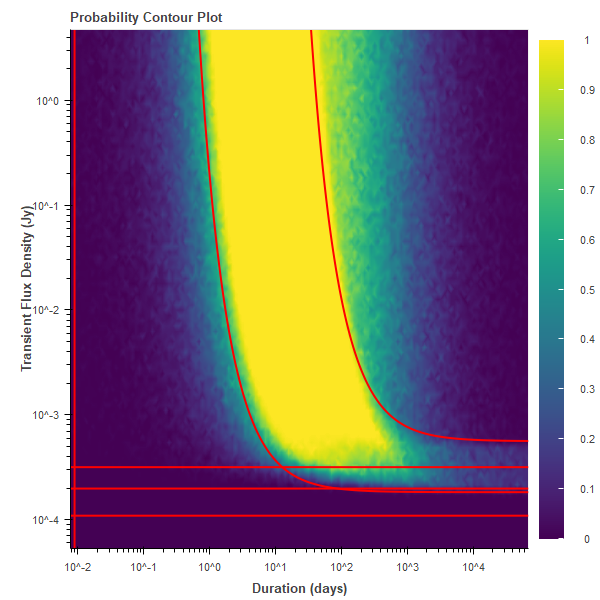
\includegraphics[width=4in]{output_fred_ProbContour.png}
				
		\label{FRED}
	\end{center}
\end{figure}
\subsubsection{Tophat}
One of the lines plotted is the longest duration that a transient could have and still fall into a gap in the observation intervals. This corresponds to the length of time just after the first observation and just before the last observation. The other line is the longest possible duration a source could have before being detected as a constant source. This corresponds to the duration from the beginning of the first observation until the end of the last observation.


\begin{figure}[H] 
	\begin{center}
		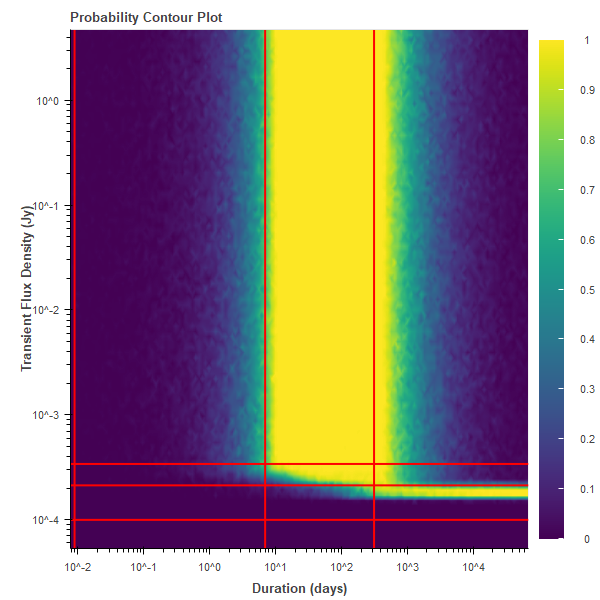
\includegraphics[width=4in]{output_tophat_ProbContour.png}
		
		\label{tophat}
	\end{center}
\end{figure}
\subsubsection{Gaussian}
Once again we enforce a limit that guides us to limiting cases:
\[f_{int} = S_{obs}\]
 First, we use the equation for integrated flux we had previously:
\[f_0 \frac{\tau}{10(t_4-t_3)}\sqrt{2\pi}\Delta F_{CDF} =  S_{obs}\]
Inserting the variables:
\[f_0 \frac{\tau}{10(t_4 - t_3)}\sqrt{2\pi}(F_{CDF}(t_8; \tau/2,\tau/10) -F_{CDF}(t_9; \tau/2, \tau/10)) =  S_{obs}\]

We repeat the same scenarios as outlined above in the FRED case:
\begin{itemize}
	\item It is bright enough to almost be detected from the beginning of the first observation until the last observation \begin{itemize}
		\item $t_8$ is the time of the end of observations, $t_{end}$; minus the start of the first observation, $t_{start}$; minus the duration of an observation, $(t_4-t_3)$; plus the duration, $\tau$
		\item $t_9$ is the time of the end of observations,  $t_{end}$; minus the start of the first observation, $t_{start}$; plus the duration
	\end{itemize}
	\item It is bright enough to be detected from the start of observations, but short enough to perhaps fall in the gap before the next observation\begin{itemize}
		\item $t_8$ is the duration of a gap, $\tau_{gap}$; plus the duration of a observation, $(t_4-t_3)$
		\item $t_9$ is the duration of a gap, $\tau_{gap}$; plus the duration of a observation, $(t_4-t_3)$; plus the duration of another observation, $(t_4-t_3)$
	\end{itemize} 
\end{itemize}
For the first case we have:
\[f_0  =  S_{obs}\frac{10(t_4 - t_3)}{\sqrt{2\pi}\tau}(F_{CDF}(t_{\text{end}}-t_{\text{start}}-(t_4-t_3)+ \tau; \tau/2,\tau/10) -F_{CDF}(t_{\text{end}} - t_{\text{start}} + \tau; \tau/2, \tau/10))^{-1}\]
For the second case we have:
\[f_0  =  S_{obs}\frac{10(t_4 - t_3)}{\sqrt{2\pi}\tau}(F_{CDF}(\tau_{gap} + (t_4-t_3); \tau/2,\tau/10) -F_{CDF}(t_{\text{end}} - t_{\tau_{gap}} + 2(t_4-t_3); \tau/2, \tau/10))^{-1}\]
In the figure below, we see only part of the line from the second case. It seems that there may be some additional conditions that are not imposed.
\begin{figure}[H] 
	\begin{center}
		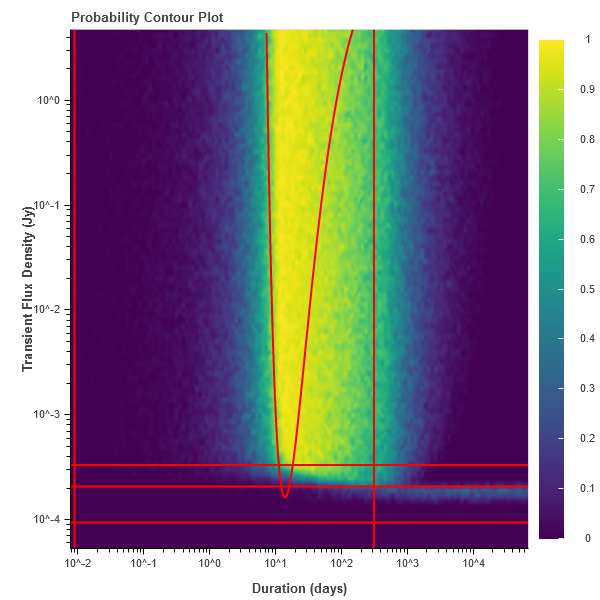
\includegraphics[width=4in]{output_gaussian_ProbContour.png}
		
		\label{gaussian}
	\end{center}
\end{figure}
\end{document}
